\documentclass{sig-alternate-05-2015}
\usepackage[l2tabu,orthodox]{nag}
\usepackage[utf8x]{inputenc}
\usepackage[british]{babel}
\usepackage[babel=true]{microtype}
\usepackage{amsmath}
\usepackage[all]{onlyamsmath}
\usepackage{newtxtext}
\usepackage{newtxmath}
\usepackage{upquote}
\usepackage{graphicx}
\usepackage{url}
\usepackage[caption=false]{subfig}
\usepackage{booktabs}
\usepackage{bytefield}
\usepackage{listings}
\usepackage{algorithm}
\usepackage{algpseudocode}
\usepackage{color}
\usepackage{balance}
\usepackage{tabularx}
\usepackage{rotating}
\usepackage{tikz}
\usepackage{xspace}   %MF
\usepackage{enumitem} %MF

\makeatletter
\global\let\tikz@ensure@dollar@catcode=\relax
\makeatother

\newcommand{\fail}{\tikz\draw[red,fill=red] (0,0) circle (.5ex);}
\newcommand{\pass}{\tikz\draw[green,fill=green] (0,0) circle (.5ex);}
\newcommand{\okay}{\tikz\draw[orange,fill=orange] (0,0) circle (.5ex);}


\newcommand{\ie}{{i.e.,}\xspace}
\newcommand*\rot{\rotatebox{90}}

\newcommand{\todo}[1]{\textbf{\textcolor{red}{To do -- #1}}}

%==================================================================================================
% The following information gets written into the PDF file information:
\pdfinfo{
  /Title        (Implementing Real-time Transport Services over an Ossified Network)
  /Author       (Stephen McQuistin, Colin Perkins, and Marwan Fayed)
  /Subject      (Real-time Transport Protocols)
  /Keywords     (Transport Services, TCP, TCP Hollywood)
  /CreationDate (D:20160516000000+01'00')
  /ModDate      (D:20160516000000+01'00')
  /Creator      (LaTeX)
  /Producer     (pdfTeX)
}
%==================================================================================================
\begin{document}
\title{Implementing Real-Time Transport Services over an Ossified Network}
\numberofauthors{3}
\author{
  \alignauthor
    Stephen McQuistin\\
    \affaddr{University of Glasgow, UK}\\
    \email{sm@smcquistin.uk}
  \alignauthor
    Colin Perkins\\
    \affaddr{University of Glasgow, UK}\\
    \email{csp@csperkins.org}
  \alignauthor
    Marwan Fayed\\
    \affaddr{University of Stirling, UK}\\
    \email{mmf@cs.stir.ac.uk}
}

\CopyrightYear{2016} 
\setcopyright{acmlicensed}
\conferenceinfo{ANRW '16,}{July 16 2016, Berlin, Germany}
\isbn{978-1-4503-4443-2/16/07}\acmPrice{\$15.00}
\doi{http://dx.doi.org/10.1145/2959424.2959443}

\maketitle
%==================================================================================================
\begin{abstract}

% Four sentences:
%  - State the problem
%  - Say why it's an interesting problem
%  - Say what your solution achieves
%  - Say what follows from your solution

Real-time applications require a set of transport services not currently
provided by widely-deployed transport protocols. Ossification prevents the
deployment of novel protocols, restricting solutions to protocols using
either TCP or UDP as a substrate. We describe the transport services
required by real-time applications. We show that, in the short-term (i.e.,
while UDP is blocked at current levels), TCP offers a feasible substrate
for providing these services. Over the longer term, protocols using UDP
may reduce the number of networks blocking UDP, enabling a shift towards
its use as a demultiplexing layer for novel transport protocols.

\end{abstract}
%==================================================================================================
\begin{CCSXML}
  <ccs2012>
    <concept>
      <concept_id>10003033.10003039.10003040</concept_id>
      <concept_desc>Networks~Network protocol design</concept_desc>
      <concept_significance>500</concept_significance>
    </concept>
    <concept>
      <concept_id>10003033.10003039.10003048</concept_id>
      <concept_desc>Networks~Transport protocols</concept_desc>
      <concept_significance>500</concept_significance>
    </concept>
  </ccs2012>
\end{CCSXML}

\ccsdesc[500]{Networks~Protocol design}
\ccsdesc[500]{Networks~Transport protocols}

\printccsdesc

\keywords{Transport protocols; real-time multimedia applications}
%==================================================================================================
\section{Introduction}

% A good paper introduction is fairly formulaic. If you follow a simple set
% of rules, you can write a very good introduction. The following outline can
% be varied. For example, you can use two paragraphs instead of one, or you
% can place more emphasis on one aspect of the intro than another. But in all
% cases, all of the points below need to be covered in an introduction, and
% in most papers, you don't need to cover anything more in an introduction.
%
% Paragraph 1: Motivation. At a high level, what is the problem area you
% are working in and why is it important? It is important to set the larger
% context here. Why is the problem of interest and importance to the larger
% community?

Real-time applications are increasingly
%important
present in the Internet.
%We want to make it easier to write these applications
Such applications should be easier to program, while also improving
the quality of experience for users.
 %of those applications
by lowering latency and increasing robustness.
%In this, we are
This limitations of standard Internet transport protocols makes this a
challenging target. Moreover, the ossified nature of the network makes
it increasingly difficult to deploy new transports.

% Paragraph 2: What is the specific problem considered in this paper? This
% paragraph narrows down the topic area of the paper. In the first
% paragraph you have established general context and importance. Here you
% establish specific context and background.

In practice, only UDP and TCP are widely usable in the Internet,
since remaining protocols are blocked by firewalls and other
middleboxes. UDP exposes the best-effort IP packet delivery service,
offering the flexibility to develop new protocols. The high costs
associated involve defining completely new protocol mechanisms. In
contrast TCP mechanisms are well defined, consisting of sophisticated
congestion control coupled with a reliable, ordered, byte stream API.
These are proven suitable for many applications, but are inappropriate
for real-time traffic. While both protocols may be used for real-time
applications, neither really provides the right services and API. This
forces each application to re-invent or re-interpret mechanisms that
should be provided by the transport. The increased costs and
complexity of doing so raise barriers to innovation.

% Paragraph 3: "In this paper, we show that...". This is the key paragraph
% in the introduction - you summarize, in one paragraph, what are the main
% contributions of your paper, given the context established in paragraphs
% 1 and 2. What's the general approach taken? Why are the specific results
% significant? The story is not what you did, but rather:
%  - what you show, new ideas, new insights
%  - why interesting, important?
% State your contributions: these drive the entire paper.  Contributions
% should be refutable claims, not vague generic statements.

In this paper we identify and present the appropriate set of transport
services and APIs for real-time applications, and demonstrate their
merit by implementing a proof-of-concept. We show that it is possible
to realise real-time services and APIs in the context of both TCP and
UDP, despite the limitations imposed by their legacies, and by
middleboxes, and ossification of the network.  Initial experiments
with our implementation suggest that
%to show that, despite network ossification,
the network has the flexibility to deploy new transport protocols, provided care
is taken to reinterpret application and transport layer boundaries that respect
conventional UDP and TCP.
%and deploy those new transports in the context of TCP and UDP.

% Paragraph 4: What are the differences between your work, and what others
% have done? Keep this at a high level, as you can refer to future sections
% where specific details and differences will be given, but it is important
% for the reader to know what is new about this work compared to other work
% in the area.

% Our contributions
In doing so we make three main contributions. First, we make explicit
the needs of real-time applications, as well as the appropriate
transport services and APIs to support those needs. Second, we
illustrate an example realisation of those transport services on the
current Internet, in the context of UDP and TCP deployments. Finally,
we present initial measurement results that suggest the proposed
mechanisms ought to be usable in the public Internet.

% Paragraph 5: "We structure the remainder of this paper as follows." Give
% the reader a road-map for the rest of the paper. Try to avoid redundant
% phrasing, "In Section 2, In section 3, ..., In Section 4, ... ", etc.

We begin in Section \ref{sec:services} by discussing transport
services for real-time applications, and outlining the common
conceptual API that those applications use. This is followed in
Section \ref{sec:ossification} by a review of deployment
considerations for new protocols, caused by ossification of the
network. Section \ref{sec:partial} considers, in particular, how TCP
reliability semantics can evolve within the constraints of the
existing infrastructure. The semantics are realised and put into
practice in Section \ref{sec:realising}.
% outlines how the transport services we have identified can be
% realised in practical networks.
Finally, Section \ref{sec:related} discusses related work, and Section
\ref{sec:conclusions} concludes.

%==================================================================================================
\section{Real-time Transport Services}
\label{sec:services}

In the IETF, the Transport Services (TAPS) working group is chartered to
(1) develop a taxonomy of \emph{transport services}, that is, to identify the
features that comprise, and can be combined to form, complete transport
protocols; and (2) to develop an abstract API for applications to request
desirable services, allowing the system to select an appropriate transport
protocol based on application needs. It is hoped that this will loosen the
coupling between application and transport, so enabling deployment of new
transport protocols.

Table \ref{tab:services} summarises the transport services discussed in this
Section, and required for real-time multimedia applications.
%--------------------------------------------------------------------------------------------------
\subsection{Timing and Transport Services}

The work in TAPS provides a vocabulary for discussing the components of
transport protocols.  The vocabulary is useful when discussing the needs of
real-time applications, and the protocols to support them.

Timing is the most salient feature of real-time applications. Since their data
must be conveyed with real-time demands, they all have some concept of a
\emph{deadline}. Data that fails to present within the deadline is otherwise
useless.
% Deadlines may be short or long.
The `slack' in a deadline depends on the application. Interactive applications,
such as telephony, video conferencing, or telepresence, require low end-to-end
latency. Their deadlines for presenting the media, \ie playing the audio and
displaying the video frame, range from tens to a few hundred milliseconds.
Non-interactive application deadlines associated with broadcast and on-demand
programming are on the order of seconds.
% , such as broadcast TV, may have deadlines on the order of seconds,
% or even tens of seconds for on-demand programming.

% % When compared to conventional real-time systems, networked multimedia
% % deadlines are neither soft nor hard.
% Networked multimedia deadlines are unusual when compared to other real-time
% systems. They are simultaneously flexible and strict: flexible in that the exact
% value of the deadline is typically not important, provided it is of the right
% order-of-magnitude for the application, but strict in that any particular
% deadline provides a hard cut-off, after which the data is useless.
It is useful to distinguish between networked multimedia deadlines and
deadlines in conventional real-time systems. A multimedia deadline is neither
soft, since arrivals played after a deadline contribute to poor experience; nor
are deadlines hard, since occasional missed messages can be tolerated.

\subsection{Partial Reliability}
In a best-effort network, deadlines
constrain packet delivery service to \emph{partial reliability}.
%The network has non-zero probability of losing any particular packet.
For example, when used to repair loss, the limits of forward error correction
imply some probability that packet will be non-recoverable. By contrast,
retransmissions used to recover from loss have potentially unbounded delay
(since any retransmission may itself be lost).
% These probabilities can be estimated, to give probabilistic constraints on
% loss and delay, but will be non-zero. Accordingly, to meet deadlines the
Accordingly, a transport protocol that meets deadlines should provide partial
reliability, acknowledging that it may be unable to deliver all data by its
deadline.

Many real-time applications run over TCP today, though TCP offers no partial
reliability service. TCP's full reliability can lead to play-out stalls
when the application is blocked by retransmissions that take too
long. These stalls are one of the primary causes of poor user experience in
streaming applications.
% , and are directly caused by the lack of partial reliability in TCP.
For the applications under scrutiny, a missed frame that fails to deliver by its
deadline is much less disruptive than a stall in play-out.

\subsection{Message-oriented Dependencies}

The combination of deadlines and partial reliability leads to \emph{dependency
management} as an important transport service.
% There is no point in sending data that cannot be used because it depends on
% previous data that was not received.
In particular, data should never be sent when it relies on a previous
transmission that was never received. Providing this service is complicated by
the two ways in which data can be \emph{useful} to applications: it may itself
be played out, or it may be needed as part of the application's decoding chain.
Interdependencies between frames of video exist within a number of codecs,
including MPEG-1 \cite{le1991mpeg}, and newer codecs such as H.264
\cite{wiegand2003overview}. As an example, we consider MPEG-1 video:
I-frames are independent, while P- and B-frames contain only the changes 
since the previous frame (P) or between frames (B), and so are dependent on
the successful arrival of other frames. An I-frame may not arrive in time
to be played out, but may need to be sent to ensure that dependent P- and
B-frames are useful. 

In the context of both deadlines and dependencies coupled with packet loss, partial reliability
requires application-level framing \cite{clark:1990:architecture} to
make the best use of payload data. At the transport
layer, this implies a \emph{message oriented} service, that
maintains application data unit (ADU) boundaries.

Message orientation may also be used to construct a \emph{sub-stream} service.
Many multimedia applications make use of multiple data streams. For example, a
simple IPTV application will maintain separate audio and video stream. These
could be sent across multiple transport-layer connections, but overheads can be
reduced by multiplexing these flows on a single connection.

\subsection{Connection and Congestion Control}

We note the importance of congestion control. %Clearly,
Historically real-time applications needed an isochronous channel,
and needed to avoid subjected to congestion control. This is impractical on the
Internet. Further, while some applications are non-adaptive or constant bitrate,
an increasing number are either or both of adaptive and variable bitrate.
Users would be better served by applications that adapt to available bandwidth.

We note that a connection-oriented transport is a lesser, but useful,
requirement.
% for many real-time multimedia applications.
Indeed, flexibility to
change the destination within a call is beneficial for
applications that support mobile users, or for some forms of multiparty session.
However, to support NAT traversal and to help dynamically manage firewall
pinholes, it is often desirable, though not necessary, for the transport to be connection oriented. We
believe these concerns outweigh the benefits of connectionless transport, and so
add a requirement for connection oriented service. Similarly, while not strictly
needed by the applications, it is beneficial if the transport provides a
keep-alive service to refresh NAT and firewall bindings if the application goes
silent.

%--------------------------------------------------------------------------------------------------
\subsection{Abstract API}

Given the set of transport services outlined in Table \ref{tab:services},
we sketch an abstract API in  Table \ref{tab:api}. The primitives divide
into four categories:

\begin{itemize}
  \item Hosts setup and tear-down sockets using the \texttt{socket()}
    and \texttt{close()} functions, as in the standard Berkeley sockets
    API.

  \item The connection primitives are the same as those of TCP sockets.
    Servers \texttt{bind()} to a particular address and port, then
    \texttt{listen()} for and \texttt{accept()} incoming connections.
    Clients \texttt{connect()} to a server.

   \item Once the connection is established, the receiver
     then indicates its media play-out delay, in milliseconds, via
     the \texttt{set\_po\_delay()} call. This specifies the time that the
     application will buffer data, to compensate for network timing jitter,
     before it is rendered to the user. The play-out delay is fed back to
     the sender host, for use as part of the media deadline estimation.

  \item Finally, message-oriented data transmission is exposed by the
    \texttt{send\_message()} and \texttt{recv\_message()} functions.
    These expose a partially reliable message delivery service to the
    application, framing data such that either a complete message is
    delivered, or it is lost in its entirety.

\end{itemize}

    It is instructive to compare the partially reliable send and receive
    functions to their Berkeley Sockets API counterparts. The
    \texttt{send\_message()} call takes four additional parameters. These are 1)
    a message sequence number, that can be used to re-order messages and detect
    message loss; 2) a relative deadline, which is combined with an estimate of
    the current round-trip-time, and the time that the message has spent in the
    sending buffer, to determine if a message will arrive in time to be
    played-out; 3) the message sequence number of any message on which this
    depends, for example, of a video I-frame on which a P-frame is predicted;
    and 4) a sub-stream identifier, used, for example, to differentiate audio,
    video, sub-title, control, and repair streams.

    The \texttt{recv\_message()} call returns the sequence number, dependency
    information, and sub-stream identifier along with any received message,
    allowing the receiver to direct it to the correct decoding queue.

%    \todo{relate this to the transport services described earlier}



A message that won't arrive within its lifetime is considered to have
\emph{expired}. A message is also considered to have expired if its
message sequence number dependency, \texttt{depends\_on},
%on which a message depends, . If the message depends on a message that has expired, then it too is considered to have
has expired. A partial reliability service follows
from this deadline and dependency service: messages will be reliably
transmitted until they expire.

\begin{table}
  \scriptsize
  \centering
  \begin{tabular}{ll}
    \toprule
      Transport Service     & Requirement \\
    \midrule
      Deadlines             & Core        \\
      Partial reliability   & Core        \\
      Dependencies          & Core        \\
      Message-oriented      & Core        \\
      Sub-streams           & Core        \\
      Congestion controlled & Core        \\
      Connection oriented   & Subsidiary  \\
      Keep-alive            & Subsidiary  \\
    \bottomrule
  \end{tabular}
  \caption{Transport services for real-time multimedia}
  \label{tab:services}
\end{table}

\begin{table*}
  \small
  \centering
  \begin{tabularx}{\textwidth}{llll}
    \toprule
      Transport Service            & Function & Parameters                                     & Return Value(s) \\
    \midrule
                                   & \texttt{socket}
                                              & \texttt{af} -- Address family                  & Socket descriptor \\
                                   &          & \texttt{st} -- Socket type & \\
                                   & \texttt{close}
                                              & \texttt{sd} -- Socket descriptor               & 0 (success), -1 (error) \\
    \midrule
      Connection oriented          & \texttt{bind}
                                              & \texttt{sd} -- Socket descriptor               & 0 (success), -1 (error) \\
                                   &          & \texttt{addr} -- Address to bind to & \\
                                   &          & \texttt{addrlen} -- Length of \texttt{addr} & \\
                                   & \texttt{listen}
                                              & \texttt{sd} -- Socket descriptor               & 0 (success), -1 (error) \\
                                   & \texttt{accept}
                                              & \texttt{sd} -- Listening socket descriptor     & Connection socket descriptor \\
                                   &          & \texttt{addr} -- Address of peer & \\
                                   &          & \texttt{addrlen} -- Length of \texttt{addr} & \\
                                   & \texttt{connect}
                                              & \texttt{addr} -- Address to connect to         & 0 (success), -1 (error) \\
                                   &          & \texttt{addrlen} -- Length of \texttt{addr} & \\
    \midrule
      Deadlines                    & \texttt{set\_po\_delay}
                                              & \texttt{delay} -- Playout delay (in ms)        & 0 (success), -1 (error) \\
    \midrule
      Message oriented             & \texttt{send\_message}
                                              & \texttt{sd} -- Socket descriptor               & Number of bytes sent \\
                                   &          & \texttt{buf} -- Message data & \\
                                   &          & \texttt{len} -- Length of message data & \\
                                   &          & \texttt{seq\_num} -- Sequence number & \\
      Deadlines                    &          & \texttt{deadline} -- Relative deadline of message (in ms) & \\
      Dependencies                 &          & \texttt{depends\_on} -- \texttt{seq\_num} of dependency & \\
      Sub-streams                  &          & \texttt{substream} -- Substream identifier & \\
                                   & \texttt{recv\_message}
                                              & \texttt{sd} -- Socket descriptor               & Number of bytes received \\
                                   &          & \texttt{buf} -- Buffer for message data        & Substream identifier \\
                                   &          & \texttt{len} -- Size of \texttt{buf} & \\
    \bottomrule
  \end{tabularx}
  \caption{Outline transport API for real-time applications. Return values
  shown are for successful calls; in all cases, -1 is returned in the event
  of an error}
  \label{tab:api}
\end{table*}

It is to be noted that this API is not dissimilar to the PR-SCTP abstract
API, which provides \textit{timed reliability}, using a ``lifetime''
specified by the application.
%\todo{CSP: check this}

%==================================================================================================
\section{Innovation and Ossification}
\label{sec:ossification}

The Internet architecture, in principle, allows free innovation at the
transport layer, provided the underlying network (IP) layer is unchanged.
Routers should inspect the source addresses of packets to perform network
ingress filtering \cite{rfc:2827}, and the destination addresses to route
packets to the correction destination, but should not inspect their
contents. This is not, of course, how the real network operates.

There are performance and security benefits that can be attained by
adding transport-layer functionality \emph{within} the network. For
example, a firewall can better protect the network if it can detect payload
anomalies.

The implication of this reality is that it is difficult to deploy new
transport protocols. The installed base of NATs, firewalls, and other
middleboxes is such that packets that do not look like TCP or UDP are
unlikely to pass the network. We may innovate all we like, provided the
transport of the future looks like TCP or UDP to middleboxes.\footnote{
  This is inconvenient, certainly, but is not necessarily a bad thing.
  The Internet is critical infrastructure. It support emergency services,
  healthcare applications, infrastructure components, financial services,
  and so on, many of which are essential to the functioning of society.
  Making changes to this type of infrastructure \emph{should} require
  careful backwards compatibility \cite{mcquistin:2015:reinterpreting}.
}

UDP is the obvious base for future protocol development, since it provides
minimal additional services over the IP layer, allowing great flexibility
in innovation for protocols tunnelled on top. Provided middleboxes do not
inspect the payload too carefully, the only real cost to innovation, when
compared to a native transport protocol running over IP, is a few bytes of
additional header. Examples in this space include RTP \cite{rfc:3550}, one
of the most widely deployed real-time transport protocols; the WebRTC Data
Channel \cite{draft-ietf-rtcweb-data-channel-13}, which tunnels
peer-to-peer SCTP associations over a DTLS association over UDP; and QUIC
\cite{draft-tsvwg-quic-protocol-02}, which provides a modern alternative
to TCP, implemented over UDP.

Despite these advantages, UDP can be problematic as a substrate for new
protocol development. UDP traffic is blocked by some enterprise firewalls,
and some in the operations community have a strong distrust of UDP-based
protocols and applications \cite{draft-byrne-opsec-udp-advisory-00}. In
part this is due to ignorance. Outside specific niches, such as DNS, UDP
has not been widely used in enterprise environments, and hence is widely
misunderstood. Blocking the unknown is a rational response. In addition,
UDP traffic has been widely used as a component of distributed denial of
service (DDoS) attacks, leading some to install blanket blocks of UDP as
a safety measure (blanket blocking, rather than the more targeted blocks
used when TCP traffic is used in DDoS attacks, are justified using the
argument that UDP is not widely used).
These issues are slowly changing, as UDP-based applications penetrate the
enterprise consciousness, but not clear that UDP is universally available
(Google report 90-95\% of endpoints are reachable with QUIC
running over UDP \cite{roskind2013quic}, but it is not clear that the set
of hosts running their Chrome browser is representative of all Internet
environments).

Beyond the availability of UDP, it is often necessary to use TCP because
HTTP is being used at the application-layer. For real-time systems, this
is likely to be an HTTP adaptive streaming (HAS) protocol, such as
MPEG-DASH or Apple's HLS. Using TCP as a substrate enables the use of these
protocols, allowing applications to benefit from the existing
infrastructure that supports them.

TCP is a more complex choice for innovation. It is a more sophisticated
protocol than UDP, with complex headers, and a protocol state machine
that mandates much more behaviour and is widely understood, and policed,
by in-network middleboxes. This does not mean that TCP cannot evolve, or
form the basis for new transport services. Rather, it means that any
innovation or development must be done carefully, paying very careful
attention to backwards compatibility.

We identify a number of places where TCP can evolve with comparative
freedom. These include congestion control, the end-point API, and data
segmentation. If care is taken, there is also the possibility to change
the reliability semantic.

The TCP congestion control algorithm is executed by the end points, and
can be changed, provided the new version requires no new information to
be exchanged.
%\todo{expand, and discuss how this evolution has occurred to date}
We note that, while standardised TCP congestion control has followed the
goal of maximising throughput at the expense of latency and variability,
this is not required by the protocol. TCP Vegas \cite{brakmo:1994:tcp-vegas}
is perhaps the best known approach that changes these constraints, with a
delay-based algorithm that reduces latency. It would also be possible to
implement alternatives that seek stability, or compatibility with the
dictates of a video codec, rather than traditional ``TCP Friendly''
congestion control -- even if implemented within TCP.
\todo{Review A: Show how the API supports alternative congestion control
algorithms.}
\todo{Review B: Alternatives might have deployment challenges (e.g.,
fairness between delay and loss based algorithms).}

The API that is exposed to applications using TCP is invisible from the
network, and can be changed. Relaxing the API to enable out-of-order
delivery of segments is trivial: segments are delivered to the application
in the order that they arrive, with their TCP sequence attached. The TCP
sequence number can be passed to the application using the existing
Berkeley sockets API, either with the received data, or using
\texttt{getsockopt()}. Out-of-order delivery is not useful when using a
byte-stream abstraction, and so the API should be further modified to
provide a message-oriented abstraction. The Berkeley sockets API already
supports such an abstraction for datagram protocols.

These changes could address many of the transport service needs for
real-time applications, but still leave a critical issue of how to improve
timing behaviour. Specifically, how to enable partial reliability for TCP,
after which it is possible to layer-on support for managing deadlines and
dependencies.

\todo{Review A: Section 3 should also note that connectionless send and
receive already work on connection-oriented sockets}

%==================================================================================================
\section{Partial Reliability and TCP}
\label{sec:partial}

Partial reliability (i.e., reliability conditional on timing and dependency
information) can be implemented by relaxing TCP's reliability guarantee.
The implication of this is that we need to offer a message-oriented
abstraction to applications. If the arrival of a segment cannot be
guaranteed, then it is not possible to offer a byte stream abstraction.

To offer a message-oriented abstraction, the boundaries between each
message must be maintained between sender and receiver. This means that a
framing mechanism is required: it is not sufficient to send each message in
a single segment, as this mapping will not necessarily be maintained by the
network. A framing marker is added to the start and end of each message
before transmission. An encoding algorithm is used to escape all occurrences
of the framing marker within the message data. This process does not impact
on the data that can be sent or received by applications.

In order to maintain compatibility with middleboxes, offering partial
reliability requires using \emph{inconsistent retransmissions}. This means
that the mapping between message data and TCP sequence numbers is no longer
static: a given TCP sequence number may be relate to different messages at
different times. Therefore, an application-level sequence number is
required to allow messages to be uniquely identified.
\todo{Review B: Inconsistent retransmissions are not well introduced. Should
be more explicit, and earlier.}

When a TCP segment is to be retransmitted, the mapping between its
sequence number and application-level sequence numbers is used to determine
which messages within the segment are to be retransmitted. A liveness check
is performed on these messages, to determine that (i) the message will
arrive on time to be played out; and (ii) the message does not depend on an
expired message. For (i), we combine the time that the message has spent in
a sending queue, with an estimate of the round-trip time and the current
play-out delay. This is then compared against the lifetime of the message,
as expressed by the application. For (ii), we maintain metadata about
sequence numbers that have expired, and check this metadata for the
dependency expressed by the application.

This mechanism -- inconsistent retransmissions -- is visible to middleboxes
on the network that are performing payload inspection. These middleboxes
may interpret this behaviour relating to an attack. For example, a
man-on-the-side attack exhibits similar behaviour, where a malicious host
is injecting data into an existing TCP flow. As a result, our connection
may be disrupted. Honda \emph{et al}.\ \cite{honda:2011:extend-tcp} conducted
experiments across 135 paths on the Internet, to determine support for
inconsistent retransmissions. They observed that the majority of paths
delivered inconsistent retransmissions successfully. On Port 80 (HTTP), the
original segment was delivered on 7\% of paths tested. Only one connection
reset was observed.

We conducted further deployment experiments using
inconsistent retransmissions \cite{mcquistin2016hollywood}, testing all
major UK providers. The results are shown in Table \ref{tab:deployability}.
We found that 100\% of tested fixed-line networks
delivered inconsistent retransmissions successfully. However, the delivery
of the original segment is common on cellular networks, with only 25\% of
tested networks delivering inconsistent retransmissions successfully and
reliably. The behaviour observed when evaluating cellular networks was
consistent with that of a transparent, split-connection TCP cache. Segments
were lost, but were retransmitted (with the IP address of the sender) by a
middlebox in the network. It is likely that these caches are deployed close
to the wireless link, given its relatively high rate of non-congestive
loss.

\begin{table}
  \scriptsize \centering
    \begin{tabular}{llcc}
    \toprule
    & ISP & Port 4001 & Port 80 \\ \midrule
    \textbf{Fixed-line} & Andrews \& Arnold & \pass & \pass \\
    & BT & \pass & \pass \\
    & Demon & \pass & \pass \\
    & EE & \pass & \pass \\
    & Eclipse & \pass & \pass \\
    & Sky & \pass & \pass \\
    & TalkTalk & \pass & \pass \\
    & Virgin Media & \pass & \pass \\ \midrule
    \textbf{Cellular} & EE & \okay & \okay \\
    & O2 & \okay & \okay \\
    & Three & \pass & \pass \\
    & Vodafone & \pass & \okay \\
    \bottomrule
    \end{tabular}
  \caption[]{Deployability of inconsistent retransmissions, where \pass \thinspace
  indicates successful delivery, \okay \thinspace indicates delivery of the original
  data, and \fail \thinspace indicates connection failure (none observed)}
  \label{tab:deployability}
\end{table}

These deployment experiments suggest that our protocol should be
flexible: inconsistent retransmissions might not be delivered, and we should
handle reception of the original segment. If the protocol detects that
inconsistent retransmissions are not being delivered, they
can be disabled for the connection. Further, if a connection reset occurs,
then the connection should be retried with the mechanism disabled.

Use of inconsistent retransmissions may interact negatively with
caching and re-segmenting middleboxes, resulting in the corruption of
messages between sender and receiver. A message may be formed from the
original message, and an inconsistent retransmission, given how the
mechanism uses the TCP sequence space. To protect against this, a checksum
must be attached to each message, to allow the receiver to verify its
integrity. The role of a checksum may also be fulfilled by using a secure
transport, such as DTLS \cite{rfc:6347}.

\todo{Review A: Section 4 should have a forward reference to section 5}
%==================================================================================================
\section{Realising Transport Services}
\label{sec:realising}

While further measurement studies are required to confirm the ability to
deploy wire-visible changes to TCP (such as inconsistent retransmissions),
we have shown that we can provide all of the transport services needed by
real-time applications, using either TCP or UDP.

Evidence that these services can be deployed above UDP exists in the form
of the WebRTC data channel \cite{draft-ietf-rtcweb-data-channel-13} and
QUIC protocol \cite{draft-tsvwg-quic-protocol-02}.
The former is a peer-to-peer protocol, comprising an SCTP association
running over DTLS, itself running over a UDP flow negotiated via an SDP
\cite{RFC4566} offer/answer exchange \cite{RFC3264} as part of a WebRTC
session \cite{jennings:2013:rtcweb} (WebRTC media uses RTP
over UDP also, further showing the utility of UDP-based data).
This has been deployed in popular web browsers, with global deployment, and
demonstrated to be effective.  The latter is implemented by Google in their
Chrome browser, and used as an alternative to TCP has a significant
fraction of web traffic downloads from their domain.

% The API shown in Table \ref{tab:api} is largely similar to that PR-SCTP,
% which has seen real-world deployments within the WebRTC protocol,
% demonstrating that we can layer these services above UDP.

Deployments using UDP are popular, and work well. However, as described in
Section \ref{sec:ossification}, there are also reasons for providing these
services over TCP, since there are a significant fraction of networks that
block UDP traffic. It is clearly possible to run real-time traffic over
TCP, as demonstrated by applications such as NetFlix or the BBC iPlayer
that comprise the majority of Internet traffic. However, TCP has a
inconvenient API that imposes lots of work on application developers, and
introduces higher than desired latency. We have shown how to address these
issues, and provide the full set of transport services we propose in
Section \ref{sec:services} in previous work, with our TCP Hollywood
proposal \cite{mcquistin2016hollywood}.

\begin{figure}[t]
 \centering
 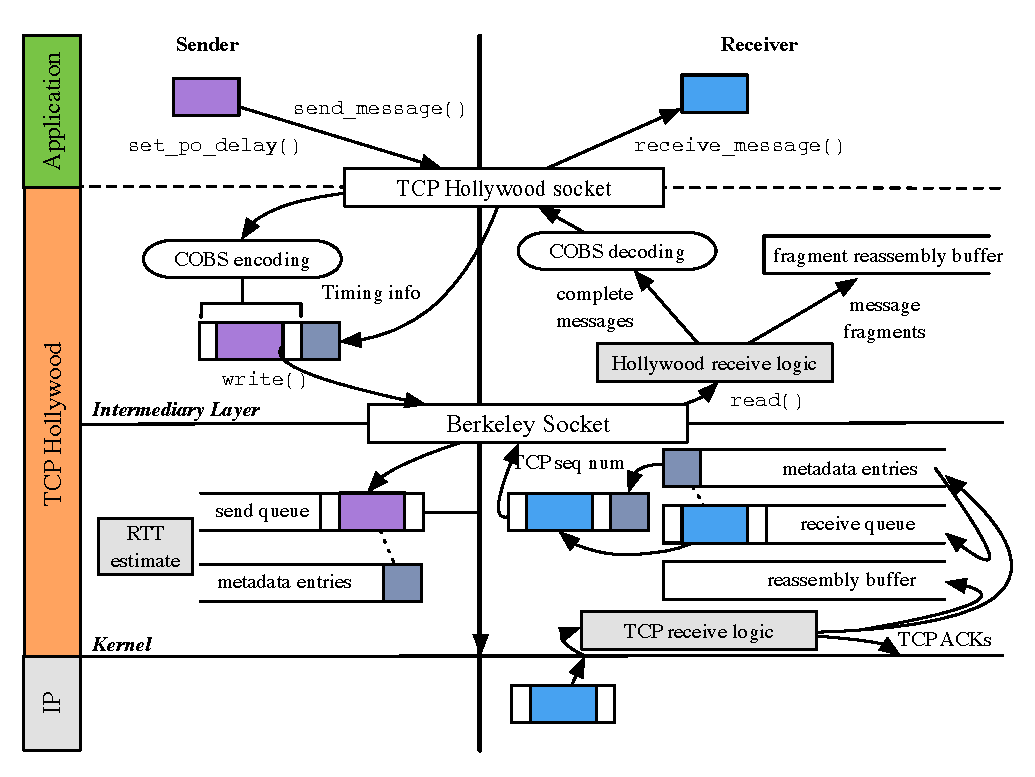
\includegraphics[scale=0.45]{figures/tcp-hollywood.pdf}
  \caption{TCP Hollywood architecture}
\label{diagram:tcp-hollywood}
\end{figure}

The architecture of TCP Hollywood is shown in Figure
\ref{diagram:tcp-hollywood}. TCP Hollywood implements all of the services
described in Section \ref{sec:services}, splitting functionality across
an intermediary layer in user-space, and a set of modifications to the
kernel. This split allows applications to program against one API, whether
or not the kernel modifications are available: the intermediary layer
functions in both cases.

At the sender, applications pass messages (using an API similar to that
given in Table \ref{tab:api}) to the intermediary layer, with their
metadata, including deadline and dependency information. At the
intermediary layer, COBS encoding \cite{CB97COBS} is used to escape all
zero bytes in the message data, allowing them to be used as framing
markers. The message's metadata is then attached to the encoded and framed
message, before being passed to the kernel using the standard Berkeley
sockets API.

At the kernel, the message data is queued in TCP's sending buffer, while
the metadata is held in a separate structure. Nagle's algorithm, designed
to coalesce smaller writes into larger segments, is disabled to minimise
latency. As segments are (re-)transmitted, their deadlines and dependencies
are checked to ensure that the message will be useful on arrival. In the
current version of TCP Hollywood, the dependency check does not overrule
the deadline check: only data that can be played out will be sent. If the
message does not pass the liveness check, the next message in the queue
that is live will be sent instead. If this is a retransmission, then
inconsistent retransmissions will be used: the replacement message will be
sent with the same TCP sequence number as the original.

At the receiver, segments are passed to the kernel, where they are
initially processed as under standard TCP: duplicate acknowledgements are
generated for out-of-order segments, for example. After this, a metadata
entry is created, and placed in FIFO queue. When the intermediary layer
reads from the socket, it receives the segment associated with the
metadata entry at the head of the queue, with its TCP sequence number
attached.

At the intermediary layer on the receiver, incoming segments are scanned
for complete messages (i.e., data between two zero bytes), which are
decoded and passed to the application. Any message fragments are buffered,
alongside their TCP sequence number, awaiting the arrival of the remainder
of the message. Once the message has been reassembled, it is decoded, and
delivered to the application.
\todo{Review B: Head-of-line blocking problem not introduced, so not clear
why this mechanism is needed.}
% TCP Hollywood inherits standard TCP's congestion control mechanism.
% Clearly, being a loss-based algorithm, this is not appropriate for
% real-time applications.
% \todo{discuss how we need to change TCP congestion control}

Taken together, the wide experiences with the WebRTC Data Channel and QUIC
demonstrate that the transport services necessary to support real-time
traffic could be deployed running over UDP. Our work prototyping the TCP
Hollywood protocol, and earlier measurements by Honda \emph{et al}.\
\cite{honda:2011:extend-tcp} also suggest that deployment over TCP is
possible.

%==================================================================================================
\section{Related Work}
\label{sec:related}

% This should come near the end, and focussing on discussing how your work
% relates to that of others. Any relevant related work should have been
% cited already, so this is not a list of related work, it's a discussion
% of how that work relates.
%
% Why not put related work after the introduction? 1) because describing
% alternative approaches gets between the reader and your idea; and 2)
% because the reader knows nothing about the problem yet, so your
% (carefully trimmed) description of various technical trade-offs is
% absolutely incomprehensible.
%
% When writing the related work:
%  - Give credit to others where it's due; this doesn't diminish the
%    credit you get from your paper.
%  - Acknowledge weaknesses in your approach.
%  - Ensure related work is accurate and up-to-date

Related changes to TCP are made by Minion protocol \cite{nowlan:2012:minion},
that uses TCP as a substrate to provide an unordered, message-oriented
service to applications, enabling some of the transport services described
in Section \ref{sec:services}, but without support for partial reliability,
deadlines, and dependencies.
Time-Lined TCP (TLTCP) \cite{mukherjee:2000:timelines} similarly provides a
message-oriented service, but allows applications to attach a time-line
to messages. Messages are (re-)transmitted as under standard TCP within
their time-line, after which they are discarded. The mechanism by which
this service is provided (introducing gaps in the sequence space) hinders
deployment.

QUIC \cite{draft-tsvwg-quic-protocol-02} demonstrates that similar services
can be provided by a new protocol running over UDP, while \cite{RFC6773} and
\cite{draft-ietf-rtcweb-data-channel-13} demonstrate that existing protocols,
DCCP and SCTP, can also be effectively tunnelled over UDP. Fallback to TCP
is discussed in this paper, and on our previous work \cite{mcquistin2016tcp}.

%==================================================================================================
\section{Conclusions}
\label{sec:conclusions}

The standard transport protocols, TCP and UDP, are not well-suited for
real-time applications. Both can be made to work, but the existence of
numerous papers exploring how to make media play-out over TCP reliable,
and almost as extensive a collection discussing UDP-based protocol design,
suggests that this is difficult to do well. To make effective use of the
network, and simplify real-time application design and implementation, we
need to deploy new transport services and protocols that allow innovative
applications to be developed by users who are not experts in transport 
protocol design. We discussed requirements for such a new transport, in
the context of the TAPS framework, and outlined a straw-man abstract API,
in Section \ref{sec:services}.

It seems likely that the right long-term approach for doing this is to
repurpose UDP as a demultiplexing layer for higher-layer protocols. We can
then deploy an appropriate transport protocol framework as a user-space
library, that can be reused as appropriate. In the short-term, however, 
there are sufficient networks that block UDP, that any new transport
protocol needs to be able to run over TCP. Sections \ref{sec:ossification}
and \ref{sec:partial} discuss how this can be done, and suggest from some
initial measurement studies that this may be feasible to deploy. Section
\ref{sec:realising} considers prototypes that present such services over
UDP, and presents our initial prototype demonstrated for TCP-based use.

The challenge for the future is in combining such techniques below a common
API, so that an application can transparently switch between UDP-based and
TCP-based transport, depending on what is supported by the underlying
network. This is the promise of the TAPS API, that we have shown ought to
be feasible for real-time applications.

% Making effective use of the TAPS concept to support real-time multimedia
% requires making significant changes to the TCP specification and API, if
% such applications are to be able to fall-back to TCP from UDP, and still
% achieve their performance needs.

%==================================================================================================
%\section{Acknowledgements}
%
% Acknowledge funding sources.
%
%==================================================================================================
\balance
\bibliographystyle{abbrv}
\bibliography{paper}
\end{document}
% vim: set ts=2 sw=2 tw=75 et ai:
